% !TeX root = origami-math-he.tex

\chapter{האקסיומות}\label{c.axioms}

\section{אקסיומה 1}\label{s.ax1}


\textbf{אקסיומה} 
נתונות שתי נקודות שונות
$p_1=(x_1,y_1)$, $p_2=(x_2,y_2)$,
קיים קיפול יחיד
$l$
העובר דרך שתיהן.

%\begin{figure}[H]
\begin{center}
\selectlanguage{english}
\begin{tikzpicture}[scale=1.2]
\draw[step=10mm,white!50!black,thin] (-1,-1) grid (8,6);
\draw[thick] (-1,0) -- (8,0);
\draw[thick] (0,-1) -- (0,6);
\foreach \x in {0,...,8}
  \node at (\x-.2,-.2) {\sm{\x}};
\foreach \y in {1,...,6}
  \node at (-.2,\y-.3) {\sm{\y}};
\coordinate (P1) at (2,2);
\coordinate (P2) at (6,4);
\draw[very thick,dashed] ($(P1)!-.75!(P2)$) -- node[very near end,below] {$l$} ($(P1)!1.5!(P2)$);
\fill (P1) circle(2pt) node[above left] {$p_1$};
\fill (P2) circle(2pt) node[above left] {$p_2$};

\draw[very thick,dotted,->,bend left=30] (2,5) to (4,1);
\end{tikzpicture}
\end{center}
%\end{figure}

\textbf{פיתוח משוואת הקיפול}

המשוואה של הקיפול 
$l$
מתקבלת מהקואורדינטות של 
$p_1$
ו-%
$p_2$:
השיפוע הוא המנה של הפרשי הקואורינטות ונקדות החיתוך עם ציר ה-%
$y$
מתקבלת מ-%
$p_1$:
\begin{equation}
\selectlanguage{english}
y - y_1 = \disfrac{y_2-y_1}{x_2-x_1}(x-x_1)\,.
\end{equation}

\vspace*{-3ex}
%\newpage

\textbf{דוגמה}

נסמן
$p_1=(2,2), p_2=(6,4)$. 
המשוואה של 
$l$  היא:
\begin{form}{2}
y-2&=&\disfrac{4-2}{6-2}(x-2)\\
y&=&\disfrac{1}{2}x+1\,.
\end{form}

%%%%%%%%%%%%%%%%%%%%%%%%%%%%%%%%%%%%%%%%%%%%%%%%%%%%%%%%%%%%%%%%
\newpage

\section{אקסיומה 2}\label{s.ax2}


\textbf{אקסיומה} 
נתונות שתי נקודות שונות
$p_1=(x_1,y_1)$, $p_2=(x_2,y_2)$,
קיים קיפול יחיד 
$l$
המניח את
$p_1$
על
$p_2$.

%\begin{figure}[H]
\begin{center}
\selectlanguage{english}
\begin{tikzpicture}[scale=1.2]
\draw[step=10mm,white!50!black,thin] (-1,-1) grid (8,6);
\draw[thick] (-1,0) -- (8,0);
\draw[thick] (0,-1) -- (0,6);
\foreach \x in {0,...,8}
  \node at (\x-.2,-.2) {\sm{\x}};
\foreach \y in {1,...,6}
  \node at (-.2,\y-.3) {\sm{\y}};
\coordinate (P1) at (2,2);
\coordinate (P2) at (6,4);
\coordinate (mid1) at ($(P1)!.5!(P2)$);
\coordinate (mid2) at ($(P1)!.5!(P2)+(-1,2)$);

\draw[rotate=30] (mid1) rectangle +(8pt,8pt);

\draw[very thick,dotted] (P1) -- (P2);
\draw[very thick,dashed] ($(mid1)!-1.4!(mid2)$) -- node[very near end,left,yshift=-12pt] {$l$} ($(mid1)!1.4!(mid2)$);
\fill (P1) circle(2pt) node[above left] {$p_1$};
\fill (P2) circle(2pt) node[above left] {$p_2$};

\draw[very thick,dotted,->,bend right=50] (2,1.8) to (6,3.8);
\end{tikzpicture}
\end{center}
%\end{figure}

\textbf{פיתוח משוואת הקיפול}

הקיפול 
$l$
הוא האנך האמצעי של
$\overline{p_1p_2}$.
השיפוע שלו הוא ההופכי השלילי של השיפוע של הקו המחבר את
$p_1$
ו-%
$p_2$.
$l$
עובר דרך נקודת האמצע בין שתי הנוקדות:
\begin{equation}
\selectlanguage{english}
y - \disfrac{y_1+y_2}{2} = -\disfrac{x_2-x_1}{y_2-y_1}\left(x-\disfrac{x_1+x_2}{2}\right)\,.\label{eq.midpoint1}
\end{equation}

\textbf{דוגמה}

נסמן
$p_1=(2,2), p_2=(6,4)$.
המשוואה של 
$l$
היא:
\begin{form}{2}
y-\left(\disfrac{2+4}{2}\right)&=&-\disfrac{6-2}{4-2}\left(x-\left(\disfrac{2+6}{2}\right)\right)\\
y&=&-2x+11\,.
\end{form}

%%%%%%%%%%%%%%%%%%%%%%%%%%%%%%%%%%%%%%%%%%%%%%%%%%%%%%%%%%%%%%%%
\newpage

\section{אקסיומה 3}\label{s.ax3}


\textbf{אקסיומה} 
נתונים שני קווים
$l_1$
ו-%
$l_2$,
קיים קיפול
$l$
המניח את
$l_1$ 
על
$l_2$.

%\begin{figure}[H]
\begin{center}
\selectlanguage{english}
\begin{tikzpicture}[scale=1.2]
\draw[step=10mm,white!50!black,thin] (-1,-1) grid (8,7);
\draw[thick] (-1,0) -- (8,0);
\draw[thick] (0,-1) -- (0,7);
\foreach \x in {0,...,8}
  \node at (\x-.2,-.2) {\sm{\x}};
\foreach \y in {1,...,7}
  \node at (-.2,\y-.3) {\sm{\y}};
\coordinate (L1a) at (2,2);
\coordinate (L1b) at (4,6);
\draw[thick] (L1a) -- node[very near start,right,yshift=-4pt] {$l_1$} (L1b);
\draw[thick,dotted,name path=l1] ($(L1a)!-.75!(L1b)$) -- ($(L1a)!1.25!(L1b)$);
\coordinate (L2a) at (7,1);
\coordinate (L2b) at (4,4);
\draw[thick] (L2a) -- (L2b);
\draw[thick,dotted,name path=l2] ($(L2a)!-.3!(L2b)$) -- node[very near start,above,xshift=4pt,yshift=2pt] {$l_2$} ($(L2a)!2!(L2b)$);
\path [name intersections = {of = l1 and l2, by = {PM}}];
\fill (PM) circle(2pt) node[below left,xshift=-9pt,yshift=-7pt] {$p_i$};

\node[above right,xshift=10pt,yshift=4pt] at (PM) {$\alpha$};
\node[below right,xshift=10pt] at (PM) {$\alpha$};
\node[above left,xshift=-3pt,yshift=12pt] at (PM) {$\beta$};
\node[above right,xshift=-3pt,yshift=12pt] at (PM) {$\beta$};

\coordinate (B1a) at (0,4.13);
\coordinate (B1b) at (6,5.1);
\draw[very thick,dashed] ($(B1a)!-.15!(B1b)$) -- node[very near start,above] {$l_{f_1}$}  ($(B1a)!1.35!(B1b)$);

\coordinate (B2a) at (3,6.73);
\coordinate (B2b) at (4,.57);
\draw[very thick,dashed] ($(B2a)!-.05!(B2b)$) -- node[very near end,right,xshift=4pt,yshift=6pt] {$l_{f_2}$} ($(B2a)!1.25!(B2b)$);

\draw[very thick,dotted,->,bend right=50] (6,2.2) to (4.5,6.7);
\draw[very thick,dotted,->,bend left=50] (6.2,1.6) to (1.8,1.3);
\end{tikzpicture}
\end{center}
%\end{figure}

\textbf{פיתוח משוואת הקיפול עבור קווים מקבילים}

אם הקווים מקבילים, 
$l_1$
הוא
$y=mx+b_1$
ו-%
$l_2$
הוא
$y=mx+b_2$.
הקיפול הוא הקו המקביל ל-%
$l_1,l_2$ 
וחצי המרחק ביניהם:
$y=mx+\disfrac{b_1+b_2}{2}$.


\textbf{פיתוח משוואת הקיפול עבור קווים נחתכים}

אם הקווים נחתכים,
$l_1$ 
הוא
$y=m_1x+b_1$
ו-%
$l_2$
הוא
$y=m_2x+b_2$.


$p_i=(x_i,y_i)$,
נקודת החיתוך של שני הקווים, הוא:
\begin{form}{1.8}
m_1x_i+b_2&=&m_2x_i+b_2\\
x_i &=& \disfrac{b_2-b_1}{m_1-m_2}\\
y_i &=&m_1x_i+b_1\,.
\end{form}

\newpage

\textbf{דוגמה}

נסמן ב-%
$l_1$
את הקו
$y=2x-2$,
ונסמן ב-%
$l_2$
את הקו
$y=-x+8$.
נקודת החיתוך היא:
\begin{form}{2}
x_i&=&\disfrac{8-(-2)}{2-(-1)}=\disfrac{10}{3}\approx 3.33\\
y_i &=& 2\cdot\disfrac{10}{3}-2=\disfrac{14}{3}\approx 4.67\,.
\end{form}

\textbf{פיתוח משוואת השיפוע של חוצה הזווית}

שני קווים יוצרים זווית בנקודות החיתוך, למעשה, שני זוגות של זוויות קודקודיות. הקיפולים הם חוצי הזווית שלהן.

אם הזווית של
$l_1$
יחסית לציר ה-%
$x$
הוא
$\theta_1$ 
והזווית של 
$l_2$
יחסית לציר ה-%
$x$
הוא
$\theta_2$,
אזי קיפול הוא הקו היוצר זווית של
$\theta_b=\disfrac{\theta_1+\theta_2}{2}$
יחסית לציר ה-%
$x$.

$\tan\theta_1=m_1$
ו-%
$\tan\theta_2=m_2$
נתונים ו-%
$m_b$,
השיפוע של חוצה הזווית, הוא:
\[
m_b=\tan\theta_b=\tan\disfrac{\theta_1+\theta_2}{2}\,.
\]
פיתוח המשוואה מחייב שימוש בשוויונות הטריגונומטריות:%
\footnote{%
פיתוח המשוואות הללו נתון בנספח%
~\ref{a.tangent}.}
\begin{form}{2.2}
\tan(\alpha_1+\alpha_2)&=& \disfrac{\tan\alpha_1+\tan\alpha_2}{1-\tan\alpha_1\tan\alpha_2}\\
\tan \disfrac{\alpha}{2}&=& \disfrac{-1\pm\sqrt{1+\tan^2\alpha}}{\tan \alpha}\,.
\end{form}
תחילה נמצא את
$m_s$,
השיפוע של
$\theta_1+\theta_2$:
\[
m_s=\tan(\theta_1+\theta_2)= \disfrac{m_1+m_2}{1-m_1m_2}\,.
\]
אחר כך נמצא את 
$m_b$,
השיפוע של חוצה הזווית:
\begin{form}{2.1}
m_b&=& \tan\disfrac{\theta_1+\theta_2}{2}\\
&=&\disfrac{-1\pm\sqrt{1+\tan^2(\theta_1+\theta_2)}}{\tan (\theta_1+\theta_2)}\\
&=&\disfrac{-1\pm\sqrt{1+m_s^2}}{m_s}\,.
\end{form}

\newpage

\textbf{דוגמה}

עבור הקווים
$y=2x-2$
ו-%
$y=-x+8$,
השיפוע של חוצה הזווית הוא:
\begin{form}{2.1}
m_s=\disfrac{2+(-1)}{1-(2 \cdot -1)}=\disfrac{1}{3}\\
m_b=\disfrac{-1\pm\sqrt{1+(1/3)^2}}{1/3}=-3\pm \sqrt{10}\approx -6.16,\; 0.162\,.
\end{form}

\textbf{פיתוח משוואת הקיפול}

נפתח את המשוואה של הקיפול
$l_{f_1}$
באיור עם שיפוע חיובי. אנו יודעים את הקואורדינטות של נקודת החיתוך של שני הקווים
$m_i=\left(\disfrac{10}{3},\disfrac{14}{3}\right)$:
\begin{form}{2}
\disfrac{14}{3} &=& (-3+\sqrt{10}) \cdot \disfrac{10}{3} + b\\ b&=&\disfrac{44-10\sqrt{10}}{3}\\
y&=& (-3+\sqrt{10})x + \disfrac{44-10\sqrt{10}}{3}\approx 0.162x+4.13\,.
\end{form}


%%%%%%%%%%%%%%%%%%%%%%%%%%%%%%%%%%%%%%%%%%%%%%%%%%%%%%%%%%%%%%%%
\newpage

\section{אקסיומה 4}\label{s.ax4}


\textbf{אקסיומה} 
נתונים נקודה
$p_1$
וקו
$l_1$,
קיים קיפול יחיד
$l$
הניצב ל-%
$l_1$
שעובר דרך
$p_1$.
%\begin{figure}[H]
\begin{center}
\selectlanguage{english}
\begin{tikzpicture}[scale=1.2]
\draw[step=10mm,white!50!black,thin] (-1,-1) grid (8,7);
\draw[thick] (-1,0) -- (8,0);
\draw[thick] (0,-1) -- (0,7);
\foreach \x in {0,...,8}
  \node at (\x-.2,-.2) {\sm{\x}};
\foreach \y in {1,...,7}
  \node at (-.2,\y-.3) {\sm{\y}};
\coordinate (L1a) at (2,0);
\coordinate (L1b) at (5,6);
\draw[thick] (L1a) -- node[very near start,right,yshift=-4pt] {$l_1$} ($(L1a)!1.15!(L1b)$);
\fill (2,6) circle (2pt) node[above right] {$p_1$};
\draw[thick,dashed] (0,7) -- node[very near end,above right] {$l$} (8,3);
\coordinate (intersection) at (4.4,4.8);
\draw[rotate=-30] (intersection) rectangle +(8pt,8pt);

\draw[very thick,dotted,->,bend left=50] (5.4,6.3) to (3.7,3);
\end{tikzpicture}
\end{center}
%\end{figure}

\textbf{פיתוח משוואת הקיפול}

נסמן את
$y = m_1x + b_1$
ב-%
$l_1$,
ונסמן
$p_1=(x_1,y_1)$. 
$l$
ניצב ל-%
$l_1$
לכן השיפוע שלו הוא
$-\disfrac{1}{m_1}$.
הקו עובר דרך
$p_1$
ונוכל לחשב את החיתוך שלו 
$b$
ולכתוב את המשוואה:
\begin{form}{2}
y_1=-\disfrac{1}{m} x_1 + b\\
b= \disfrac{(my_1+x_1)}{m}\\
y=-\disfrac{1}{m} x +\disfrac{(my_1+x_1)}{m}\,.
\end{form}
\textbf{דוגמה}

נסמן ב-%
$p_1$
את הנקודה
$(2,6)$
ונסמן ב-%
$l_1$
את הקו
$y=2x-4$.
המשוואה של הקיפול
$l$
היא:
\[
y=-\disfrac{1}{2}x + \disfrac{2\cdot 6 + 2}{2}=-\disfrac{1}{2}x + 7\,.
\]


%%%%%%%%%%%%%%%%%%%%%%%%%%%%%%%%%%%%%%%%%%%%%%%%%%%%%%%%%%%%%%%%
\newpage

\section{אקסיומה 5}\label{s.ax5}


\textbf{אקסיומה} 
נתונות נקודות
$p_1,p_2$
ונתון קן
$l_1$,
קיים קיפול
$l$
המניח את
$p_1$
מעל
$l_1$
והעובר דרך
$p_2$.

%\begin{figure}[H]
\begin{center}
\selectlanguage{english}
\begin{tikzpicture}[scale=1.1]
\draw[step=10mm,white!50!black,thin] (-1,-1) grid (9,9);
\draw[thick] (-1,0) -- (9,0);
\draw[thick] (0,-1) -- (0,9);
\foreach \x in {0,...,9}
  \node at (\x-.2,-.2) {\sm{\x}};
\foreach \y in {1,...,9}
  \node at (-.2,\y-.3) {\sm{\y}};
\coordinate (L1a) at (0,3);
\coordinate (L1b) at (8,-1);
\draw[thick] (L1a) -- node[near end,below right,xshift=8pt,yshift=-8pt] {$l_1$} (L1b);
\coordinate (P1) at (2,8);
\fill (P1) circle (2pt) node[above left] {$p_1$};
\coordinate (P2) at (4,4);
\fill (P2) circle (2pt) node[above left,yshift=4pt] {$p_2$};
\draw[thick,dotted,name path=L1] (8,-1) -- (-1,3.5);
\node[very thick,dotted,draw, name path = circle] at (P2)
    [circle through = (P1)] {};

\path [name intersections = {of = circle and L1, by = {P1P,P1PP}}];
\fill (P1P) circle (2pt) node[above left,xshift=-2pt,yshift=4pt] {$p_1'$};
\fill (P1PP) circle (2pt) node[above left,yshift=6pt] {$p_1''$};

\coordinate (f1) at (0,6);
\draw[thick,dashed] ($(f1)!-.25!(P2)$) -- node[very near end,above] {$l_{f_2}$} ($(f1)!2.25!(P2)$);
\coordinate (f2) at (0,2);
\draw[thick,dashed] ($(f2)!-.25!(P2)$) -- node[very near end,below,yshift=-2pt] {$l_{f_1}$} ($(f2)!2.25!(P2)$);

\draw[very thick,dotted,->,bend left=50] (2.2,7.8) to (-.2,3.2);
\draw[very thick,dotted,->,bend left=50] (2.4,7.85) to (6.1,.2);
\end{tikzpicture}
\end{center}
%\end{figure}

עבור זוג נקודות נתון וקו נתון, יכולים להיות אפס, אחד או שני קיפולים.

\textbf{פיתוח משוואות עבור השיקופים}

נסמן ב-%
$l$
את הקיפול העובר דרך
$p_2$,
ונסמן ב-%
$p_1'$
את השיקוף של
$p_1$
מסביב ל-%
$l$.
האורך של
$\overline{p_1p_2}$
שווה לאורך של
$\overline{p_2p_1}'$.
המקום הגיאומטרי של נקודות הנמצאות במרחק
$\overline{p_1p_2}$
\textbf{מ-}%
$p_2$
הוא המעגל שמרכזו
$p_2$
והרדיוס שלו הוא האורך
$\overline{p_1p_2}$. 
נקודות החיתוך של מעגל זה עם הקו
$l_1$
הן המקומות האפשריים עבור
$p_1'$.

נסמן
$y=m_1x + b_1$
ב-%
$l_1$,
ונסמן
$p_1=(x_1,y_1)$, $p_2=(x_2,y_2)$.
המשוואה של המעגל שמרכזו
$p_2$
עם רדיוס באורך של
$\overline{p_1p_2}$
היא:
\begin{form}{1.5}
(x-x_2)^2 + (y-y_2)^2 = r^2\\
r^2= (x_2-x_1)^2 + (y_2-y_1)^2\quad \textrm{\R{כאשר}}\,.
\end{form}
נציב את המשוואה של הקו לתוך המשוואה של המעגל:
\[
(x-x_2)^2+((m_1x+b_1)-y_2)^2=(x-x_2)^2+(m_1x+(b_1-y_2))^2=r^2\,,
\]
ונקבל משוואה ריבועית עבור קואורדינטות ה-%
$x$
של נקודות החיתוך האפשריות:
\begin{equation}
\selectlanguage{english}
x^2(1+m_1^2) \,+\, 2(-x_2+m_1b-m_1y_2)x \,+\, (x_2^2 + (b_1^2 - 2b_1y_2+y_2^2)-r^2)=0\,.\label{eq.intersections}
\end{equation}
למשוואה ריבועית יש לכל היותר שני פתרונות
$x_1',x_1''$,
ונחשב את 
$y_1',y_1''$
מ-%
$y=m_1x+b_1$.
נקודות השיקוף הן
$p_1'=(x_1',y_1'), p_1''=(x_1'',y_1'')$.

\textbf{דוגמה}

נסמן ב-%
$p_1$
את הנקודה
$(2,8)$
ונסמן ב-%
$p_2$
את הנקודה
$(4,4)$.
נסמן ב-%
$l_1$ 
את הקו
$y=-\disfrac{1}{2}x +3$.
משוואת המעגל היא:
\[
(x-4)^2 + (y-4)^2 = r^2=(4-2)^2+(4-8)^2=20\,.
\]
נציב את המשוואה של הקו לתוך המשוואה של המעגל ונפשט כדי לקבל משוואה ריבועית עבור קואורדינטות ה-%
$x$
של נקודות החיתוך )אפשר גם להשתמ משוואה%
~\L{\ref{eq.intersections}}(:
\begin{form}{1.5}
(x-4)^2 + \left(\left(-\disfrac{1}{2}x+3\right)-4\right)^2&=&20\\
\disfrac{5}{4}x^2-7x-3 &=&0\\
5x^2 -28x -12&=&0\\
(5x+2)(x-6)&=&0\,.
\end{form}
שתי נקודות חיתוך הן:
\[
p_1'=\left(-\disfrac{2}{5},\disfrac{16}{5}\right) = (-0.4,3.2)\,,\quad p_1''=(6,0)\,.
\]

\textbf{פיתוח המשוואות של הקיפולים}

הקיפולים יהיו האנכים האמצעיים של
$\overline{p_1p_1'}$
ו-%
$\overline{p_1p_1''}$.
המשוואה של אנך אמצעי נתונה על ידי משוואה%
~\L{\ref{eq.midpoint1}},
שנעתיק כאן עבור
$p_1'$:
\begin{equation}
\selectlanguage{english}
y - \disfrac{y_1+y_1'}{2} = -\disfrac{x_1'-x_1}{y_1'-y_1}\left(x-\disfrac{x_1+x_1'}{2}\right)\,.\label{eq.midpoint2}
\end{equation}

\newpage

\textbf{דוגמה}

עבור
$p_1=(2,8)$
ו-%
$p_1'=\left(-\disfrac{2}{5},\disfrac{16}{5}\right)$,
משוואת הקיפול עבור
$l_{f_1}$
היא:
\begin{form}{2}
y-\disfrac{8+(16/5)}{2}&=&-\disfrac{(-2/5)-2}{(16/5)-8}\left(x-\disfrac{2+\left(-2/5\right)}{2}\right)\\
y&=&-\disfrac{1}{2}x+6\,.
\end{form}

עבור
$p_1=(2,8)$
ו-%
$p_1''=(6,0)$,
משוואת הקיפול עבור
$l_{f_2}$ 
היא:
\begin{form}{2}
y-\disfrac{8+0}{2}&=&-\disfrac{6-2}{0-8}\left(x-\disfrac{2+6}{2}\right)\\
y&=&\disfrac{1}{2}x+2\,.
\end{form}

%%%%%%%%%%%%%%%%%%%%%%%%%%%%%%%%%%%%%%%%%%%%%%%%%%%%%%%%%%%%%%%%

\newpage

\section{אקסיומה 6}\label{s.ax6}

\textbf{אקסיומה}                          
נתונות שתי נקודות
$p_1$
ו-%
$p_2$
ונתונים שני קווים
$l_1$
ו-%
$l_2$,
קיים קיפול
$l$
המניח את 
$p_1$
על ל-%
$l_1$
ו-%
$p_2$
על ל-%
$l_2$.

%\begin{figure}[H]
\begin{center}
\selectlanguage{english}
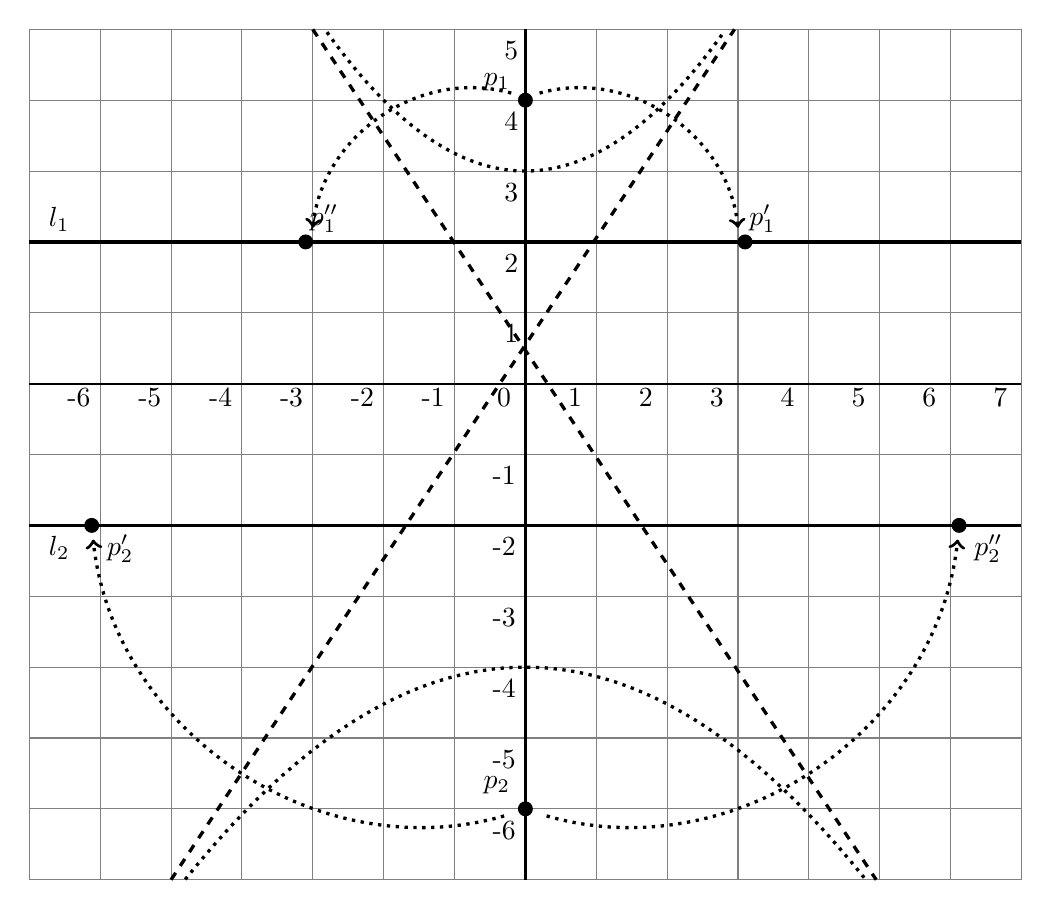
\begin{tikzpicture}[scale=.9]
\draw[step=10mm,white!50!black,thin] (-7,-7) grid (7,5);
\draw[thick] (-7,0) -- (7,0);
\draw[thick] (0,-7) -- (0,5);
\foreach \x in {-6,...,7}
  \node at (\x-.3,-.2) {\sm{\x}};
\foreach \y in {1,...,5}
  \node at (-.2,\y-.3) {\sm{\y}};
\foreach \y in {-6,...,-1}
  \node at (-.3,\y-.3) {\sm{\y}};
  
\coordinate (P1) at (0,4);
\fill (P1) circle (3pt) node[above left,xshift=-2pt] {$p_1$};
\coordinate (P2) at (0,-6);
\fill (P2) circle (3pt) node[above left,xshift=-2pt,yshift=2pt] {$p_2$};

\coordinate (P1P) at (3.1,2);
\fill (P1P) circle (3pt) node[above right,xshift=-2pt] {$p_1'$};
\coordinate (P2P) at (-6.12,-2);
\fill (P2P) circle (3pt) node[below right,xshift=2pt] {$p_2'$};

\coordinate (P1PP) at (-3.1,2);
\fill (P1PP) circle (3pt) node[above right,xshift=-2pt] {$p_1''$};
\coordinate (P2PP) at (6.12,-2);
\fill (P2PP) circle (3pt) node[below right,xshift=2pt] {$p_2''$};

\draw[very thick] (-7,2) -- node[very near start,above,xshift=-34pt] {$l_1$} (7,2);
\draw[very thick] (-7,-2) -- node[very near start,below,xshift=-34pt] {$l_2$} (7,-2);

\draw[domain=-4.8:4.8,samples=50,very thick,dotted] plot (\x,{-.13*\x*\x-4});
\draw[domain=-2.8:2.8,samples=50,very thick,dotted] plot (\x,{.25*\x*\x+3});

\draw[very thick,dashed] (-5,-7) -- (2.95,5);
\draw[very thick,dashed] (-3,5) -- (4.95,-7);

\draw[very thick,dotted,->,bend left=50] (.2,4.1) to (3,2.2);
\draw[very thick,dotted,->,bend left=50] (-.3,-6.1) to (-6.1,-2.2);

\draw[very thick,dotted,->,bend right=50] (-.2,4.1) to (-3,2.2);
\draw[very thick,dotted,->,bend right=50] (.3,-6.1) to (6.1,-2.2);
\end{tikzpicture}
\end{center}
%\end{figure}

עבור זוג נקודות נתון וזוג קווים נתון, יכולים להיות אפס, אחד, שניים או שלושה קיפולים.

קיפול המניח את 
$p_i$
על
$l_i$
הוא קו שמרחקו ל-%
$p_i$
שווה למרחקו ל-%
$l_i$.
המקום הגיאומטרי של נקודות שהן במרחק שווה מנקודה
$p_i$
ומקו
$l_i$
הוא פרבולה עם מוקד 
\L{(focus)}
$p_i$
ומדריך
\L{(directrix)}
$l_i$.
קיפול הוא כל קו המשיק לפרבולה. הצדקה מפורטת של טיעון זה נמצא בנספח%
~\ref{a.parabola}.

כדי שהקיפול יניח בו-זמנית את 
$p_1$
על ל-%
$l_1$
ו-%
$p_2$
על ל-%
$l_2$,
הוא חייב להיות משיק משותף לשתי הפרבולות.

המשוואה עבור פרבולה שרירותית די מסובכת, לכן נגביל את הדיון לפרבולה שציר ה-%
$y$
הוא ציר הסמטריה. אין כאן מגבלה משמעותית כי עבור כל פרבולה קיימים הזזה וסיבוב המעבירים אותה כך שציר הסמטריה שלה הוא ציר ה-%
$y$.

נביא גם דוגמה עם פרבולה שציר הסמטריה שלה הוא ציר ה-%
$x$.

\newpage

\textbf{פיתוח הנקודה של הקיפול}

תהי
$(0,f)$
מוקד של פרבולה עם מדריך
$y=d$.
נגדיר
$p=f-d$,
האורך )עם הסימן( של קטע הקו בין המוקד למדריך.%
\footnote{%
השתמשנו בסימון
$p_i$
עבור נקודות, כך שהשימוש כאן ב-%
$p$
עלול לבלבל, אבל סימון זה מקובל. השם הפורמלי עבור
$p$
הוא מחצית ה-%
\L{latus rectum}.}
אם קודקוד 
\L{(vertex)}
הפרבולה נמצא על ציר ה-%
$x$,
המשוואה של הפרבולה היא
$y=\disfrac{x^2}{2p}$.
כדי להזיז את הפרבולה למעלה או למטה על ציר ה-%
$y$,
כך שהקודקוד שלה היא
$(0,h)$,
יש להוסיף 
$h$
למשוואת הפרבולה:
$y=\disfrac{x^2}{2p}+h$.
\begin{center}
\selectlanguage{english}
\begin{tikzpicture}[scale=1]
\draw (-6,0) -- node[very near start,below,xshift=-32pt] {$x$-\textsf{axis}}(6,0);
\draw (0,-3) -- node[very near start,right,yshift=-20pt] {$y$-\textsf{axis}}(0,4.5);
\draw[very thick] (-6,-2) -- node[near start,below] {\textsf{directrix} $\quad y=-2$} (6,-2);
\draw[domain=-5:5,samples=50,very thick,dotted] plot (\x,{\x*\x/8+1});
\coordinate (F) at (0,4);
\fill (F) circle (2pt) node[left,xshift=-2pt,yshift=0pt] {$(0,f)=(0,4)$} node[above left,xshift=-2pt,yshift=4pt] {\textsf{focus}};
\fill (0,-2) circle (2pt);
\fill (0,1) circle (2pt) node[below left] {\textsf{vertex}} node[below left,yshift=-10pt] {$(0,1)$};
\draw[<->] (2,-1.9) -- node[fill=white] {$p=6$} +(0,5.8);
\draw[<->] (1,.1) -- node[fill=white] {$h=1$} +(0,.8);
\end{tikzpicture}
\end{center}
נגדיר
$a=2ph$
כך שמשוואת הפרבולה היא:
\begin{form}{1.5}
y=\disfrac{x^2}{2p}+\disfrac{a}{2p}\\
x^2-2py+a=0\,.
\end{form}
עבור הפרבולה באיור למעלה המשוואה היא:
\begin{form}{1}
x^2-2\cdot 6\,y + 2\cdot 6 \cdot 1=0\\
x^2-12y +12=0\,.
\end{form}
נציב את המשוואה של קו 
\textbf{שרירותי}
$y=mx+b$
במשוואה עבור הפרבולה ונקבל משוואה עבור נקודות החיתוך של הקו והפרבולה:
\begin{form}{1.5}
x^2-2p(mx+b)+a=0\\
x^2+(-2mp)x+(-2pb+a)=0\,.
\end{form}
הקו יהיה משיק לפרבולה אם ורק אם למשוואה ריבועית זו קיים 
\textbf{בדיוק}
פתרון אחד אם ורק אם הדיסקרימננטה היא אפס:
\[
(-2mp)^2\:-\:4\cdot 1\cdot (-2pb+a)=0\,.
\]
לאחר פישוט מתקבלת:
\begin{equation}
\selectlanguage{english}
m^2p^2+2pb-a=0\,.\label{eq.disc}
\end{equation}
משוואה זו עם המשתנה 
$m$ 
היא המשוואה עבור השיפועים של המשיקים לפרבולה. קיימים אינסוף משיקים כי עבור כל 
$m$,
קיים
$b$
שגורם למשיק לזוז למעלה או למטה.%
\footnote{%
פרט כמובן עבור קו המקביל לציר הסמטריה.%
}

כדי למצוא את המשיקים המשותפים לשתי הפרבולות, יש לפתור את המשוואות של שתי הפרבולות, משוואות עם שני משתנים
$m$
ן-%
$b$.

%%%%%%%%%%%%%%%%%%%%%%%%%%%%%%%%%%%%%%%%%%%%%%%%%%%%%%%%%%%%%%%%


\textbf{דוגמה}

פרבולה 1: מוקד
$(0,4)$,
מדריך
$y=2$,
קודקוד,
$(0,3)$
ו-%
$p=2$, $a=2\cdot 2\cdot 3=12$.
משוואת הפרבולה היא:
\[
\begin{array}{l}
x^2-2\cdot 2y +12=0\,.
\end{array}
\]
נציב לתוך משוואה%
~\L{\ref{eq.disc}}
ונפשט:
\[
m^2+b-3=0\,.
\]
פרבולה 2: מוקד
$(0,-4)$,
מדריך
$y=-2$,
קודקוד,
$(0,-3)$
ו-%
$p=-2$, $a=2\cdot -2\cdot -3=12$.
משוואת הפרבולה היא:
\[
x^2-2\cdot (-2)y+12=0\,.
\]
נציב לתוך משווארה%
~\L{\ref{eq.disc}}
ופשט:
\[
m^2-b-3=0\,.
\]
הפתרונות של שתי המשוואות:
\begin{form}{1.5}
m^2+b-3=0\\
m^2-b-3=0\,,
\end{form}
הם
$m=\pm\sqrt{3}\approx \pm 1.73$
ן-%
$b=0$.
המשיקים המשותפים שהם הקיפולים הם:
\[
y=\sqrt{3}x\,,\quad y=-\sqrt{3}x\,.
\]

%%%%%%%%%%%%%%%%%%%%%%%%%%%%%%%%%%%%%%%%%%%%%%%%%%%%%%%%%%%%%%%%

\textbf{דוגמה}

פרבולה 1 ללא שינוי.

פרבולה 2: מוקד
$(0,-6)$,
מדריך
$y=-2$,
קודקוד,
$(0,-4)$
ו-%
$p=-4$, $a=2\cdot -4\cdot -4=32$.
משוואת הפרבולה היא:
\[
x^2-2\cdot (-4)y +32=0\,.
\]
נציב לתוך משווארה%
~\L{\ref{eq.disc}}
ונפשט:
\[
2m^2-b-4=0\,.
\]
הפתרונות של שתי המשוואות:
\begin{form}{1.5}
m^2+b-3=0\\
2m^2-b-4=0\,,
\end{form}
הם
$m=\pm\sqrt{\disfrac{7}{3}}\approx \pm 1.53$
ו-%
$b=\disfrac{2}{3}$.
יש שני משיקים משותפים שהם קיפולים:
\[
y=\sqrt{\disfrac{7}{3}}x+\disfrac{2}{3}\,,\quad y=-\sqrt{\disfrac{7}{3}}x+\disfrac{2}{3}\,.
\]

%%%%%%%%%%%%%%%%%%%%%%%%%%%%%%%%%%%%%%%%%%%%%%%%%%%%%%%%%%%%%%%%

\textbf{דוגמה}

כעת נגדיר פרבולה שציר הסמטריה שלה הוא ציר ה-%
$x$.

פרבולה 1 ללא שינוי.

פרבולה 2: מוקד
$(4,0)$,
מדריך
$x=2$,
קודקוד,
$(3,0)$
ו-%
$p=2$, $a=2\cdot 2\cdot 3=12$.
משוואת הפרבולה היא:
\[
y^2-4x+12 = 0\,.
\]
שימו לב שזו משוואה עם 
$x$
ו-%
$y^2$
במקום
$x^2$
ו-%
$y$,
כך שלא ניתן להשתמש במשוואה%
~\L{\ref{eq.disc}}
ונצטרך לפתח את משוואות מחדש.

נציב את המשוואה עבור קו:
\begin{form}{1.5}
(mx+b)^2-4x+12=0\\
m^2x^2+(2mb-4)x+(b^2+12)=0\,,
\end{form}
נשווה את הדיסקרימננטה לאפס ונפשט:
\begin{form}{1.5}
(2mb-4)^2\:-\:4m^2(b^2+12)=0\\
-3m^2-mb+1=0\,.
\end{form}
אם ננסה לפתור את שתי המשוואות:
\begin{form}{1.5}
m^2+b-3=0\\
-3m^2-mb+1=0\,,
\end{form}
נקבל 
משוואה ממעלה שלוש במשתנה
$m$:
\begin{equation}
\selectlanguage{english}
m^3-3m^2-3m+1=0\,.\label{eq.cubic}
\end{equation}
למשוואה ממעלה שלוש יש לפחות פתרון ממשי אחד ולכן היותר שלושה פתרונות ממשיים, לכן יכול להיות אחד, שניים או שלשה משיקים משתופים. אפשר שלא יהיה אף משיק אחד אם אין פתרון לשתי המשוואות, למשל, כאשר פרבולה אחת נמצאת בתוך השנייה: 
$y=x^2$, $y=x^2+1$.

המשוואה למציאת פתרונות למשוואה ממעלה שלוש די מסובכת, לכן השתמשתי במחשבון באינטרנט וקיבלתי שלושה פתרונות:
\[
m=3.73\,, \;m=-1\,, \; m=0.27\,.
\]
אם נבחר
$m=0.27$, $b=3-m^2=2.93$,
משוואת הקיפול היא:
\[
y=0.27x+2.93\,.
\]
מהצורה של המשוואה%
~\L{\ref{eq.cubic}},
נוכל לנחש ש-%
$1$
או
$-1$
הוא פתרון:
\begin{form}{1.4}
1^3-3\cdot 1^2-3\cdot 1+1=-4\\
(-1)^3-3\cdot (-1)^2-3\cdot(-1)+1=0\,.
\end{form}
נחלק את המשוואה%
~\L{\ref{eq.cubic}}
ב-%
$m-(-1)=m+1$
ונקבל משוואה ריבועית
$m^2-4m+1$
ששורשיה הם
$2\pm\sqrt{3}\approx 3.73, 0.27$.


%%%%%%%%%%%%%%%%%%%%%%%%%%%%%%%%%%%%%%%%%%%%%%%%%%%%%%%%%%%%%%%%

\textbf{פיתוח המשוואות של השיקופים}

נפתח את המיקום של 
$p_1'=(x_1',y_1')$,
השיקוף של
$p_1=(x_1,y_1)$
מסביב למשיק
$l_t$
שהמשוואה שלה היא
$y=m_tx+b_t$.
הפיתוח זהה עבור כל משיק ועובר 
$p_2$.

כדי לשקף את
$p_1$
מסביב ל-%
$l_t$,
נמצא את הקו
$l_p$
עם המשוואה
$y=m_px+b_p$
שניצב ל-%
$l_t$
ועובר דרך
$p_1$:
\begin{form}{2}
y=-\disfrac{1}{m_t}x+b_p\\
y_1=-\disfrac{1}{m_t}x_1+b_p\\
y=\disfrac{-x}{m_t}+\left(y_1+\disfrac{x_1}{m_t}\right)\,.
\end{form}
אז נמצא את נקודת החיתוך 
$p_t=(x_t,y_t)$
של
$l_t$
ו-%
$l_p$:
\begin{form}{3}
m_tx_t+b_t=\disfrac{-x_t}{m_t}+\left(y_1+\disfrac{x_1}{m_t}\right)\\
x_t=\disfrac{\left(y_1+\disfrac{x_1}{m_t}-b_t\right)}{\left(m_t+\disfrac{1}{m_t}\right)}\\
y_t=m_tx_t+b_t\,.
\end{form}
קל למצוא את השיקוף
$p_1'$
כי נקודת החיתוך
$p_t$
היא נקודת האמצע בין
$p_1$
והשיקוף שלו
$p_1'$:
\begin{form}{2}
x_t=\disfrac{x_1+x_1'}{2}\,,\quad y_t=\disfrac{y_1+y_1'}{2}\\
x_1'=2x_t-x_1\,,\quad y_1'=2y_t-y_1\,.
\end{form}

\newpage

\textbf{דוגמה}

נסמן
$p_1=(0,4)$
ונסמן ב-%
$l_1$
את
$y=\sqrt{3}x$:
\begin{form}{2.2}
x_t=\disfrac{\left(4+\disfrac{0}{\sqrt{3}}-0\right)}{\left(\sqrt{3}+\disfrac{1}{\sqrt{3}}\right)}=\sqrt{3}\\
y_t=\sqrt{3}\sqrt{3}+0=3\\
x_1'=2x_t-x_1=2\sqrt{3}-0=2\sqrt{3}\approx 3.46\\
y_1'=2y_t-y_1=2\cdot 3 - 4 = 2\,.
\end{form}

%%%%%%%%%%%%%%%%%%%%%%%%%%%%%%%%%%%%%%%%%%%%%%%%%%%%%%%%%%%%%%%%
\newpage

\section{אקסיומה 7}\label{s.ax7}

\textbf{אקסיומה} 
נתונמ נקודה אחת
$p_1$,
ונתונים שני קווים
$l_1$,
$l_2$,
קיים קיפול
$l$
הניצב ל-%
$l_2$
שהמניח את
$p_1$
על ל-%
$l_1$.

%\begin{figure}[H]
\begin{center}
\selectlanguage{english}
\begin{tikzpicture}[scale=1.2]
\draw[step=10mm,white!50!black,thin] (-1,-1) grid (9,8);
\draw[thick] (-1,0) -- (9,0);
\draw[thick] (0,-1) -- (0,8);
\foreach \x in {0,...,9}
  \node at (\x-.2,-.2) {\sm{\x}};
\foreach \y in {1,...,8}
  \node at (-.2,\y-.3) {\sm{\y}};
  
\coordinate (P1) at (5,3);
\fill (P1) circle (2pt) node[below left] {$p_1$};

\coordinate (P1P) at (2.75,5.25);
\fill (P1P) circle (2pt) node[left,xshift=-4pt] {$p_1'$};

\draw[very thick] (1,0) -- node[very near start,right,xshift=2pt] {$l_1$} (3,6);
\draw[very thick,name path=l2] (8,3) -- node[very near start,right,xshift=-2pt,yshift=6pt] {$l_2$} (5,6);

\draw[thick,dotted] ($(1,0)!-.15!(3,6)$) -- ($(1,0)!1.34!(3,6)$);

\draw[thick,dotted] ($(8,3)!-.3!(5,6)$) -- ($(8,3)!1.65!(5,6)$);

\draw[thick,dotted] ($(P1)!-.4!(P1P)$) -- node[very near start,below,yshift=-4pt] {$l_p$} ($(P1)!1.5!(P1P)$);

\draw[very thick,dashed,name path=fold] (-.5,-.25) -- node[very near end,above,xshift=4pt,yshift=6pt] {$l$} (7.5,7.75);

\coordinate (mid) at ($(P1)!.5!(P1P)$);
\fill (mid) circle (2pt) node[below,yshift=-8pt] {$p_m$};

\path [name intersections = {of = fold and l2, by = {perp}}];
\draw[rotate=-45] (mid) rectangle +(8pt,8pt);
\draw[rotate=-45] (perp) rectangle +(8pt,8pt);


\draw[very thick,dotted,->,bend right=50] (5.1,3.2) to (3,5.2);
\end{tikzpicture}
\end{center}
%\end{figure}

\textbf{פיתוח משוואת הקיפול}

נסמן
$p_1=(x_1,y_1)$,
נסמן ב-%
$l_1$
את
$y = m_1x + b_1$ 
ונסמן ב-%
$l_2$
את 
$y=m_2x+b_2$.

הקיפול
$l$
ניצב ל-%
$l_2$,
וגם לקו
$l_p$
המכיל את
$\overline{p_1p_1'}$
והניצב ל-%
$l$,
לכן אפשר להסיק ש-%
$l_p$
מקביל ל-%
$l_2$:
\[
y=m_2x+b_p\,.
\]
$l_p$ 
עובר דרך
$p_1$
כך ש-%
$y_1=m_2x_1+b_p$
והמשוואה שלו היא:
\[
y=m_2x+(y_1-m_2x_1)\,.
\]
$p_1'=(x_1',y_1')$,
השיקוף של
$p_1$
מסביב לקיפול
$l$,
הוא נקודת החיתוך של 
$l_1$
ו-%
$l_p$:
\begin{form}{1.5}
m_1x_1'+b_1=m_2x_1'+(y_1-m_2x_1)\\
x_1'=\disfrac{y_1-m_2x_1-b_1}{m_1-m_2}\\
y_1'=m_1x_i'+b_1\,.
\end{form}
$p_m=(x_m,y_m)$,
נקודת האמצע של
$l_p$
נמצא על הקיפול
$l$:
\[
(x_m,y_m)=\left(\disfrac{x_1+x_1'}{2},\disfrac{y_1+y_1'}{2}\right)\,.
\]
הקיפול
$l$
הוא האנך האמצעי של 
$\overline{p_1p_1'}$,
וכדי לחשב את המשוואה שלו, תחילה נחשב את נקודת החיתוך של
$l$
שעובר דרך
$p_m$:
\begin{form}{2}
y_m=-\disfrac{1}{m_2}x_m+b_m\\
b_m=y_m+\disfrac{x_m}{m_2}\,.
\end{form}
המשוואה של הקיפול
$l$
היא:
\begin{form}{2}
y=-\disfrac{1}{m_2}x+\left(y_m+\disfrac{x_m}{m_2}\right)\,.
\end{form}

\vspace*{-3ex}

\textbf{דוגמה}

נסמן
$p_1=(5,3)$,
נסמן ב-%
$l_1$
את
$y=3x-3$,

ונסמן ב-%
$l_2$
את
$y=-x+11$.
 

\begin{form}{2.4}
x_1'=\disfrac{3-(-1)\cdot 5-(-3)}{3-(-1)}=\disfrac{11}{4}\\
y_1'=3\cdot \disfrac{11}{4} + (-3)=\disfrac{21}{4}\\
	p_m=\left(\disfrac{5+\disfrac{11}{4}}{2},\disfrac{3+\disfrac{21}{4}}{2}\right)=\left(\disfrac{31}{8},\disfrac{33}{8}\right)\,.
\end{form}
משוואת הקיפול היא:
\[
y=-\disfrac{1}{-1}\cdot x+\left(\disfrac{33}{8}+\disfrac{\disfrac{31}{8}}{-1}\right)=x+\disfrac{1}{4}\,.
\]

